\documentclass{article}
\usepackage[utf8]{inputenc}
\usepackage{amsmath}
\usepackage{color}
\usepackage{graphicx}
\usepackage{cases}
\title{CSC3150 Assignment2}
\author{Yu, Zhouliang 120040077 }
\date{October 2021}

\begin{document}

\maketitle

\section{Environment}
\subsection{Linux Version}
\begin{figure}[htbp]
    \centering
    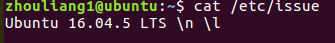
\includegraphics{Linux.png}
\end{figure}
\subsection{GCC Version}
\begin{figure}[htbp]
    \centering
    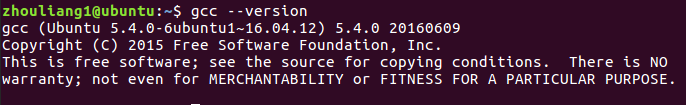
\includegraphics{GCC.png}
\end{figure}

\section{The Step to Execute The Program}
\subsection{Compile}
In the 'source' directory, type 'g++ hw2.cpp -lpthread' and enter on concole.
\subsection{Execute}
In the 'source' directory, type './a.out'

\section{The Design of My Program }
\subsection{logmove desgin}
first set the property of the logs
to make their speed vary each other, randomly generated length,
and randomly generated leftend

\begin{figure}[htbp]
    \centering
    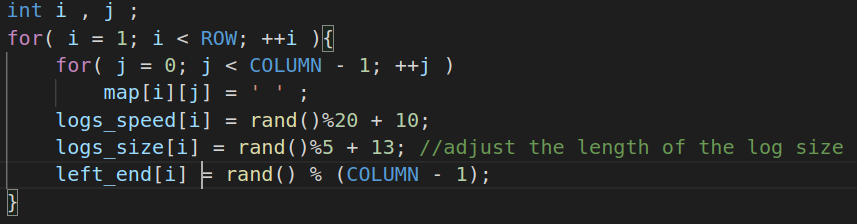
\includegraphics[width = 0.8\textwidth]{logset.png}
\end{figure}

in order for some log to move from left to right and some from right to left, I set the log on the odd row moving from left to right, while log on the even row moving from right to left

the motion of move is implemented by the operation on the array to load the left end of each log, and use mod to allow the log to go across the boundary and emerging at the other side.


\begin{figure}[htbp]
    \centering
    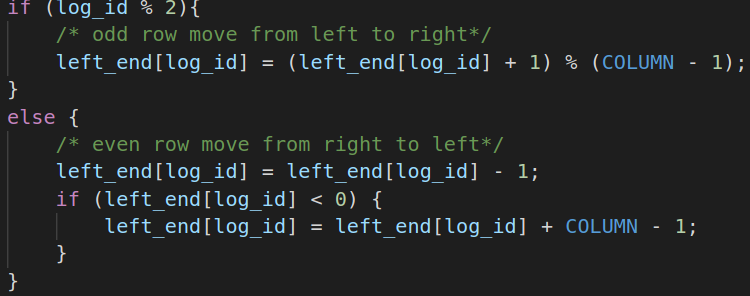
\includegraphics[width = 0.8\textwidth]{logmove.png}
\end{figure}

\subsection{create pthread and use mutex for controling frog and logs}
1. we create pthreads for each log and the downside land, their executable routine are all log\_move, to enable them to control the motion of each logs and plot maps, with arg to be '(void*) t' which can transfer to log\_id
\\
2. each pthread\_create is paired with pthread\_exit if main finishes before the threads it has created, and exit with pthread\_exit\(\) the other thread will continue to execute. otherwise, they will all automatically terminated when main finishes.
so we set a pthread\_exit at the end of main and end of log\_move
\\
3. to make the multi-thread process accomplish synchronization between threads we use pthread\_join to subroutine blocks the calling thread until the specific thread terminated 
\\
4. in order for protecting the sharing data in each thread preventing other thread to write in that thread, we use mutex to lock the pthread while its functioning

\subsection{keyboard actions capture}
in each pthread we are going to check if there is a keyboard hit, use 'getchar' to capture the action
if we press w the frog move upward, s to move downward, d to move right, a to move left, if we press q we quit
\begin{figure}[htbp]
    \centering
    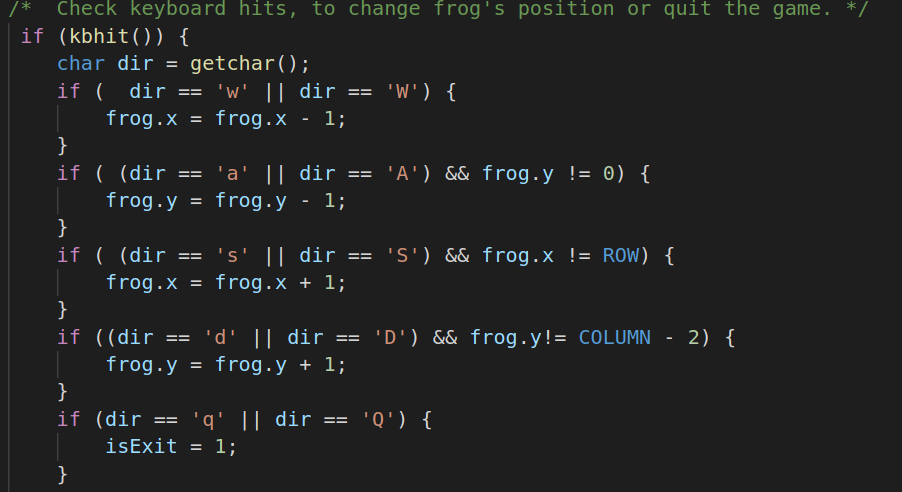
\includegraphics[width = 0.8\textwidth]{kb.png}
\end{figure}

\subsection{game status judging and message print}
we set booleans 'isWin', 'isLose','isExit' to denote the status, and in the function log\_move we are able to judge the status in each thread.
if frog falls to the rive or touches the boundary left and right, isLose will be set 1, if it goes to the other side, isWin will be set to one, if we quit, isExit will be set to 1

and if any of these status changes, we are able to print the corresponding message to the user
\begin{figure}[htbp]
    \centering
    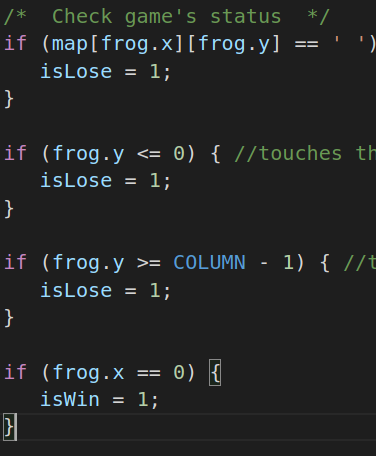
\includegraphics[height = 0.5\textwidth,width = 0.8\textwidth]{status.png}
\end{figure}
\clearpage
the print out message is
\begin{figure}[htbp]
    \centering
    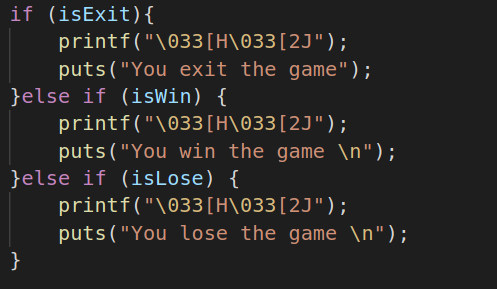
\includegraphics[width = 0.8\textwidth]{print.png}
\end{figure}

\section{bonus}

\subsection{length of logs random generating}
we use srand and random function to generate random length logs
\begin{figure}[htbp]
    \centering
    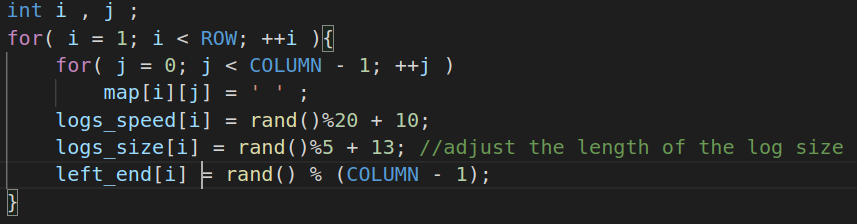
\includegraphics[width = 0.8\textwidth]{logset.png}
\end{figure}

\subsection{slide bar to adjust speed}
in my program I define a new object speed, the speed of logs can be adjust by the position of speed symbol

in my program, we can press 'K' or 'k' to increase the speed, and press 'j' or 'J' to decrease the speed

\begin{figure}[htbp]
    \centering
    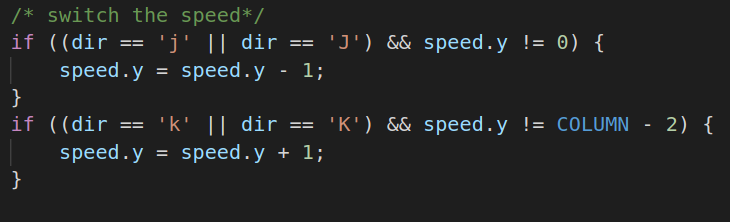
\includegraphics[width = 0.8\textwidth]{speed.png}
\end{figure}

\subsection{GUI}
This can be implemented by outer graphical library

\section{Sample Output}
\subsection{interface}
the interface of game, you will find the length of each logs is not different, because they are random generated
\begin{figure}[htbp]
    \centering
    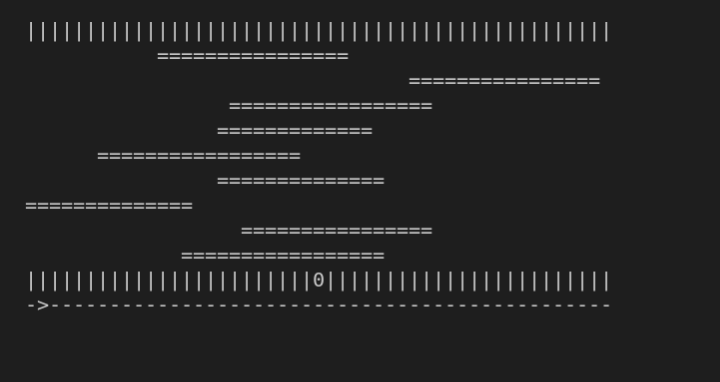
\includegraphics[width = 0.8\textwidth]{inter.png}
\end{figure}
\subsection{win}
you win the game
\begin{figure}[htbp]
    \centering
    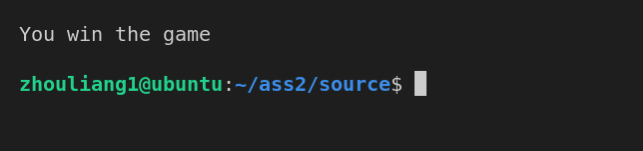
\includegraphics[width = 0.8\textwidth]{win.png}
\end{figure}
\clearpage
\subsection{lost}
you lose the game
\begin{figure}[htbp]
    \centering
    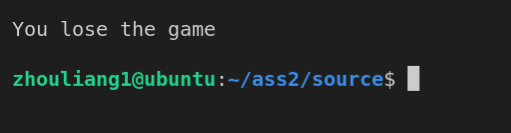
\includegraphics[width = 0.8\textwidth]{lose.png}
\end{figure}

\subsection{quit}
quit the game
\begin{figure}[htbp]
    \centering
    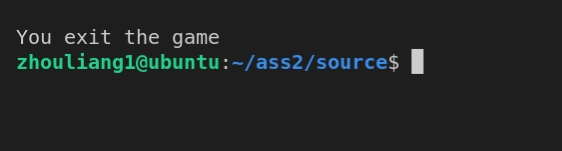
\includegraphics[width = 0.8\textwidth]{quit.png}
\end{figure}

\subsection{speed}
adjust the speed, k for right, j for left
\begin{figure}[htbp]
    \centering
    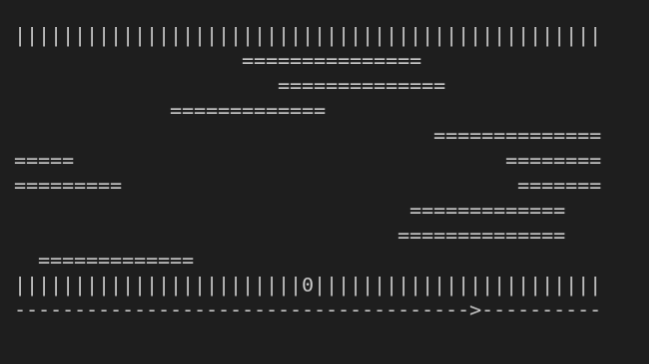
\includegraphics[width = 0.8\textwidth]{quick.png}
\end{figure}

\section{What I Learnt From the task}
\subsection{-lpthread}
Q: Why gcc does not link to the pthread by "\#include$<$pthread.h$>$", while we must use "-lpthread"
to compile the program
\\
A: 

Having \#include $<$pthread.h$>$ in your code doesn't link in the library; it only includes the header for compilation. That allows the compiler to see the various structures, function declarations, etc. included. Having -lpthread actually causes the linking to be done by the linker. So the include tells the compiler what's available, and the -lpthread actually allows the program to call the functions within the library at runtime.
\subsection{pthread\_join}
Q: Why do we use pthread\_join in multiple thread programming
\\
A: if your main thread(the thread executed by the main), exits before other threads, then it will cause bugs. With pthread\_join, the main thread is waiting until other thread exit.

\subsection{pthread\_mutex}
Q: Why do we need a mutex?
\\
A:
A mutex is a mutually exclusive flag, it acts as a gate keeper to a cection of code allowing one thread in and blocking access to al others, this ensures that code being controled will only be hit by a single thread each time, be sure to release the mutex when you are done.

reference: https://stackoverflow.com/questions/34524/what-is-a-mutex

\end{document}